~
\newpage
\section{An Introduction to Climate Change}

\subsection{The Earth is Warming (and it's Our Fault)}

In its most recent report, the United Nations' Intergovernmental Panel on Climate Change (IPCC) states:
\begin{quote}
``It is unequivocal that human influence has warmed the atmosphere, ocean and land. Widespread and rapid changes in the atmosphere, ocean, cryosphere and biosphere have occurred." \citep{ipcc1_summary}
\end{quote}
The IPCC's statement, which follows from possibly the single largest scientific endeavor in human history, is the foundation for all research, activism, and policy on climate change. This section explores this statement by summarizing why the scientific community is certain that (1) climate change has already started, and that (2) human activity is responsible for climate change. 

In daily life, we are most familiar with the weather---the day-to-day fluctuations in temperature, precipitation, cloud cover, and severe storms. Because the weather is instantaneous and observable at anytime by just taking a walk or looking out of the window, the weather is easy to notice. This is not the case with climate. Climate describes weather outcomes in the long-run. For instance, an important climate measurement is the 10-year average daily temperature. To the statistician, weather is just a random variable drawn from the climate distribution \citep{auffhammer2018quantifying}. That is, weather is like rolling a dice. It occurs in random ways and is immediately observable. Climate is like rolling a dice 10,000 times, and we can use numerical summaries to describe the full set of these 10,000 rolls, such as the value of the average roll. Although no one can accurately and easily perceive the global climate in daily life, people have long kept detailed records of the weather. By averaging together weather measurements like temperature, scientists can measure how the planet's climate has changed. 

\begin{figure}
\centering
\caption{The Plant is Warming\label{ipcc1}}
\includegraphics[width=0.6\textwidth]{figures/chapter1_figures/ipcc_fig1.png}
\vspace{1em}
\fignote[1]{Figure is from \cite{ipcc1_summary}. The vertical axis is degrees Celsius relative to global average surface temperatures from 1850--1900. The black series plots observed annual average global surface temperatures. Simulated series come from the Coupled Model Intercomparison Project Phase 6 (CMIP6). Shaded areas represent the ``very likely'' range of simulated outcomes. While it is true that there are natural, non-human reasons for the planet to warm, the figure clearly shows that these factors do not explain observed warming. Simulated warming with anthropogenic warming closely matches observed warming from the past 170 years. 
}
\end{figure}

There is absolutely no question that climate change is occurring. The black line in Figure \ref{ipcc1} displays the change in annual average global temperatures since 1850. The average global surface temperature from 2011--2020 was 1.09$^\circ$C warmer than the average global surface temperature from 1850--1900 \citep{ipcc1_summary}. The ten warmest years in the historical record have all occurred since 2010 \citep{lindsey2023climate}. 
%While calculating global temperatures is more complicated than a simple average, refuting that the planet is warming amounts to questioning whether or not thermometers actually measure the temperature. 
The Earth is warming, and even though we cannot go outside and immediately see this, it is still an empirical reality. There is also no question that climate change is driven almost exclusively by human activity. The tan series in Figure \ref{ipcc1} is simulated results using both human and natural drivers of climate, and the green series is simulated results using only natural drivers of climate. These simulations come from heavily reviewed and highly accurate climate models.\footnote{See Figure \ref{cmip6_accuracy} for an examination of the accuracy of climate models.} Natural factors alone cannot explain the rise in global temperatures. Only when we incorporate the impact of humans into climate models does the observed warming make any sense. 

As intelligently crafted as these climate models are, they are remarkably complex. This complexity makes it difficult to understand why the scientific community knows humans are responsible for contemporary climate change. Rather than unpacking the models climate scientists use to study the warming of the planet, we instead start by investigating the factors that can cause the climate to change in general.

Climate does not change without reason. The energy that warms the Earth and controls the climate comes from the Sun. Of the radiation that reaches the Earth, 30\% is immediately reflected back into space by the atmosphere and surface, 19\% is absorbed by the atmosphere, and the remaining 51\% is absorbed by the surface. When absorbed by the Earth's surface, the surface emits infrared radiation, or heat. Surface heat accounts for some of the planet's warmth, but most of this actually comes from the atmosphere \citep{csi}. When the surface emits infrared radiation, this moves out into the atmosphere. Certain particles sometimes absorb this infrared radiation and send it back to the surface. These particles are known as \emph{greenhouse gasses}. Greenhouse gases keeps some energy from leaving the planet, similar to how a blanket keeps some heat from leaving your body. This heat is not inevitably trapped on the planet, but allows the same energy to be reabsorbed by the surface before attempting to leave the atmosphere again.

The planet's global temperature is stable when the radiative energy that coming into the Earth is equal to the radiative energy that the Earth emits back into space. When the radiative energy that comes to Earth is greater than the radiative energy that leaves the Earth, then this surplus energy causes warming \citep{noaa}. This imbalance that causes changes in global temperatures is called \emph{radiative forcing} or \emph{climate forcing}.

There are several major factors that impact radiative forcing: solar irradiation, volcanic eruptions, land use, aerosols, and greenhouse gases \citep{SINGH202179}. Solar irradiation refers to the power the Sun gives to the Earth on a per unit of land basis (W/m$^2$). One important factor affecting solar irradiation is the Earth's orbit and rotation. Currently, the Earth rotates on a 23.5$^\circ$ axis, but the tilt of this axis can change over the course of millennia. This change in rotation and the subsequent climatic changes are known as Milankovitch cycles \citep{buis2020global}. These cycles also incorporate slight changes in the Earth's orbit that make it more elliptical, bringing the planet closer to the Sun during certain periods. While this does affect climate, it does so over the course of thousands of years rather than decades. Other fluctuations from the Sun have the potential to create radiative forcing and changes in the climate over somewhat shorter periods of time. For instance, reduced solar output is a leading explanation for the period of cooler climate in Europe and North America from the early 14th century to the early 19th century, an event known as the Little Ice Age \citep{little_ice}.

Other factors that can induce radiative forcing---like changes in land use, volcanic eruptions, and aerosols---do so by influencing the Earth's albedo. The Earth's albedo is the reflectivity of the planet. Recall that the Earth's atmosphere and surface reflect about 30\% of incoming radiation from the Sun. This percentage can change based on the presence of reflective and absorbent features on the surface and in the atmosphere. 

On the surface, white ice reflects radiation, and the black pavement of roads absorbs radiation, emitting back heat. Agricultural land is generally more reflective than dark forests. Land use changes like these can affect how much energy the surface absorbs or reflects, and consequently change the planet's albedo and climate. 

In the atmosphere, aerosols are the primary source of changes in the planet's albedo.Aerosols are small solid or liquid particles in the atmosphere that can influence the development of cloud cover. Around 90\% of all aerosols in the atmosphere come from natural sources including dust, sea salt, and  wildfire ash. Humans emit the remaining 10\% of aerosols. Burning coal releases sulfur dioxide and driving cars releases fine particulate matter, both aerosols. Aerosols affect climate in two ways: (1) the direct effect of either absorbing or reflecting radiation in the atmosphere, and (2) cloud formation \citep{gfdl}. Most aerosols reflect light and have a cooling effect, with the notable exception of black carbon. Black carbon absorbs light and can be particularly destructive if it coats glaciers, turning these reflective surfaces black. This is the direct effect of aerosols. The second, indirect effect of aerosols is in the creation of clouds. Clouds require aerosols in order to form. Additional aerosols in the atmosphere make cloud formation easier and can even lengthen the lifespan of a cloud. This additional cloud cover reflects radiation and keeps the surface cooler. Unfortunately many common aerosols like sulfur dioxide are dangerous for human health and create acid rain in large concentrations. 

Volcanic eruptions can also influence the planet's albedo. It is true that volcanic eruptions emit greenhouse gases like carbon dioxide. However, volcanic greenhouse gas emissions are less than one percent of all anthropogenic emissions \citep{usgs, gerlach2011volcanic}. The suggestion that higher concentrations of carbon dioxide in the atmosphere are the result of volcanic eruptions rather than human activity is utterly false. Volcanic eruptions more likely have a cooling effect on the climate (negative radiative forcing). These eruptions send large quantities of sulfur dioxide, an aerosol, into the troposphere. This creates large and long-lasting clouds that reflect solar radiation and raise the Earth's albedo. 

Lastly, greenhouse gases can create radiative forcing. Higher concentrations of greenhouse gases make it more likely that any infrared radiation emitted on the planet's surface will be re-absorbed by the atmosphere and continue to heat the surface. The most common greenhouse gas is water vapor. Water evaporates from the surface, enters the atmosphere, absorbs heat from the planet, and keeps this heat around the surface. Eventually the water vapor condenses and falls to the surface for the cycle to repeat. Although water vapor is the most common greenhouse gas, it is best understood as an accelerant of warming, not as a cause of warming. The quantity of water on the Earth is essentially fixed, and water will only evaporate and enter the atmosphere in response to some external warming. For this reason, water vapor will always act as an accelerant of warming, but never the underlying cause of warming.

\begin{figure}
	\caption{Current Carbon Dioxide Concentrations are Unprecedented \label{noaa1}}
	\centering
	\includegraphics[width=0.7\textwidth]{figures/chapter1_figures/co2_noaa.jpg}
	\vspace{1em}
	\fignote[1]{Figure is from \cite{noaa1}. Carbon dioxide concentrations are measured in parts per millions (ppm). The purple series displays carbon dioxide concentrations measured from air bubbles trapped in ice cores. The natural cycles apparent in the series are related to Milankovitch cycles. This natural variation in carbon dioxide concentrations (shown) occurs over thousands of year. Not only are current carbon dioxide concentrations greater than they have been in the hundreds of thousands of years previous, there is a clear departure from the natural cycles of carbon concentrations. On this geologic timescale, the increase in carbon dioxide within the last few generations has been essentially instantaneous. 
	}
\end{figure}

The most recognized greenhouse gas is carbon dioxide or CO$_2$. Carbon dioxide makes up the bulk of all human-induced greenhouse gas emissions and, other than water vapor, is the most prevalent greenhouse gas in the atmosphere. Figure \ref{noaa1} shows the concentration of carbon dioxide in the Earth's atmosphere over the previous hundreds of thousands of years. In all this time, the concentration of carbon dioxide in the atmosphere never exceeded 300 parts per million (ppm). In 2021, the atmospheric concentration of carbon dioxide reached 414.7 part per million. Historically, the increase in carbon dioxide is practically instantaneous, and this result is completely attributable to humans. Natural fluctuations have played out for hundreds of thousands of years---what we see today is unprecedented and undoubtedly the result of human activity, not natural causes. Elevated concentrations of greenhouse gases can keep additional infrared radiation around the surface of the Earth, warming the planet. The next section takes a closer look at greenhouse gas emissions in the US and globally. 

\begin{figure}
\centering
\caption{Warming is Driven by Human Activity \label{forcing}}
\includegraphics[width=\textwidth]{figures/chapter1_figures/ipcc_radiative_forcing.png}
\fignote[1]{Figure is from \cite{ipccAR6_radiative_forcing}. The horizontal axis displays simulated changes in global temperatures between 1750 and 2019. Temperature simulations use the estimated radiative forcing from each component combined with feedbacks from the climate system---the climate sensitivity. Dotted error bars display the 95\% confidence interval that corresponds with uncertainty with radiative forcing estimates. Solid error bars display the 95\% confidence interval that corresponds with uncertainty in both the radiative forcing and climate sensitivity estimates. The figure shows that natural radiative forcing in the middle panel is negligible, and warming is driven by human activity. Anthropogenic greenhouse gas emissions (represented by the bars labeled ``Carbon dioxide'', ``Other well-mixed greenhouse gases'', ``Ozone'', ``Stratospheric water vapor'') are responsible for the bulk of all warming. Anthropogenic aerosol emissions have a large cooling effect on the planet, by both creating cloud cover and by reflect radiation back into space. 
}
\end{figure}

These various sources, solar irradiance, land use, aerosols, volcanic eruptions, and greenhouse gases, represent a comprehensive list of the factors that could even potentially change global temperatures at the observed scale. From this point, scientists can measure how each of these factors have changed over the period we have seen warming. Incorporating some physical constants, researchers calculate the radiative forcing of each of these factors. Figure \ref{forcing} displays the results of these radiative forcing studies and makes it remarkably clear that humans are responsible for climate change. 

Natural radiative forcing from solar drivers, volcanic activity, and internal variability is not perceptible. Given how gradually these natural drivers act, it intuitively seems far-fetched that any of these could be behind the relatively rapid warming seen today. Instead, Figure \ref{forcing} shows that warming is attributable to increases in greenhouse gases like carbon dioxide, methane, nitrous oxide, and others. This warming is partially offset by increasing concentrations of aerosols. Furthermore, we know that humans are responsible for the large increases in these greenhouse gases. 

The Fourth National Climate Assessment makes the summation of all these scientific observations clear:
\begin{quote}
``Global average temperature has increased by about 1.8°F [1.0$^\circ$C] from 1901 to 2016, and observational evidence does not support any credible natural explanations for this amount of warming; instead, the evidence consistently points to human activities, especially emissions of greenhouse or heat-trapping gases, as the dominant cause." \citep{nationalar4}
\end{quote}
We call the climate change caused by humans, rather than natural forces, \emph{anthropogenic} climate change. The existence and magnitude of anthropogenic climate change is not s finding to be taken lightly, representing a shift in the planet's history into an unprecedented era where humans dominate the environment itself---the \emph{Anthropocene}.

% The planet is warming, but not quite the entire planet. The lowest level of the atmosphere that humans inhabit has warmed, but the upper layers of the atmosphere that absorb radiation from the Sun have not \citep{C2ES}. If climate change was the result of some change external to the Earth, then the stratosphere would warm as well. Without any warming in the stratosphere, we know that the warming must occur from activity on the Earth's surface. Natural activities on the surface like volcanic eruptions cannot account account for changes in temperature. These factors have largely remained unchanged over the period of warming we have already encountered, and often make such small contributions to shifts in global climate that we cannot seriously attribute climate change to these factors. Simple deduction leaves human activity as the culprit of the climate crisis.


\subsection{Greenhouse Gas Emissions: Structure \& Trends}

Anthropogenic greenhouse gas emissions drive climate change. The previous section established carbon dioxide as the preeminent greenhouse gas causing climate change, but methane and nitrous oxide both play major roles as well. Florinated gases, also called F-gases, are less common, but make up a non-negligible proportion of greenhouse gas emissions in the US and are growing at an alarming rate.

Not all these greenhouse gases are created equal. Some greenhouse gases remain in the atmosphere longer than others and absorb more infrared radiation from the Earth than others. Greenhouse gases may also react and create different greenhouse gases in the atmosphere, which themselves can have different warming effects. To improve the accounting of greenhouse gases, researchers standardize the varied warming effect of these greenhouse gases through a measure called global warming potential (GWP). GWP measures the warming effect of other greenhouse gas emissions relative to the warming effect from a ton of carbon dioxide. For instance, in the IPCC's Sixth Assessment Report, methane has a GWP of 27.9, meaning that a ton of methane emissions has the same warming effect as 27.9 tons of carbon dioxide. This metric then leads to carbon dioxide equivalent emissions, denoted CO$_2$e, a standard unit of account for different greenhouse gas.

\begin{table}
\centering
\caption{Global Warming Potential (GWP) by Greenhouse Gas \label{gwptable}}
\begin{tabular}{l c C{3cm} c}
	\hline\\[-1.8ex]
	Gas Name & Chemical Formula & Atmospheric Life (years) & GWP\\ 
	\hline\\[-1.8ex]
	Carbon dioxide & CO$_2$ &  & 1 \\
	Methane & CH$_4$ & 11.8 & 27.9\\
	Nitrous oxide & N$_2$O & 109 & 273\\
	HFC-134a & CH$_2$FCF$_3$ & 14 & 1530\\ 
	HFC-23 & CHF$_3$ & 228 & 14,600\\
	Nitrogen trifluoride & NF$_3$ & 569 & 17,400\\
	Sulfur hexafluoride & SF$_6$ & 1000 & 24,300\\
	\hline
\end{tabular}\\
\vspace{.6em}
\fignote[1]{Table adapted from \cite{ipccAR6_gwp}. Global warming potential (GWP) displayed is based on 100-year time horizon. Carbon dioxide does not have a specific atmospheric lifespan as its removal from the atmosphere is dependent on the speed of the carbon cycle. The table shows there is significant variation in the lifespan and warming effect of greenhouse gases. 
}
\end{table}

Table \ref{gwptable} lists the GWP for the most common greenhouse gases and a handful of F-gases as calculated in the IPCC's Sixth Assessment Report. Carbon dioxide is always one because it is the standard unit. Methane has a shorter atmospheric lifespan than carbon dioxide, but absorbs much more energy during this time. In the US, agriculture accounts for the largest share of methane emissions, followed closely by the mining and processing of fossil fuels \citep{epa2020overview}. Nitrous oxide emissions occur almost entirely from agriculture, particularly from the application of fertilizers and other soil management practices. These emissions linger in the atmosphere longer than methane and absorb heat better than carbon dioxide. The IPCC's  latests estimates indicate one ton of nitrous oxide equates to 273 tons of carbon dioxide. F-gases like HFC-134a (the most common hydroflorocarbon in the atmosphere), HFC-23, nitrogen trifluoride, and sulfur hexafluoride are rare. These gases emerged to replace chlorofluorocarbons following the Montreal Protocol. While these gases do not have quite the same ozone-destroying effect of their predecessors, they can have huge GWP in even small quantities. They tend to remain in the atmosphere for a much longer time and absorb far more energy than more common greenhouse gases. For this reason, F-gases are also often called high GWP gases.

\begin{figure}
\caption{US Greenhouse Gas Emissions 1990--2019\label{ghg1}}
\centering
\includegraphics[width=\textwidth]{figures/chapter1_figures/ghg_stacked.pdf}
\fignote[1]{
	Data from \cite{owidco2andothergreenhousegasemissions}. The figure displays annual emissions in the US for the three major greenhouse gases---carbon dioxide, methane, nitrous oxide---and all florinated gases. All emissions measurements are in metric tons of CO$_2$ equivalent emissions to account for differing global warming potentials. Annual US emissions have fallen since they peaked in 2007. Carbon dioxide emissions account for the vast majority of greenhouse gas emissions in the US.
}
\end{figure}

When we put all anthropogenic emissions into a common measurement, carbon dioxide equivalent, then we can compare greenhouse gas emissions and accurately evaluate the composition of greenhouse gases and the threat of certain gases relative to others. Figure \ref{ghg1} plots total greenhouse gas emissions (in millions of metric tons of carbon dioxide equivalent, CO$_2$e) in the US from 1990 to 2019 by the offending greenhouse gas. First, US greenhouse gas emissions have fallen over the past ten years. Second, it is clear why there is so much emphasis on carbon dioxide. Carbon dioxide makes up a wide majority of all anthropogenic greenhouse gas emissions in the US. Most of the recent reductions in greenhouse gas emissions are attributable to falling carbon dioxide emissions. Although they still make up just sliver of emissions, F-gases have seen the most growth over the period, up 86.3\%. 

\begin{figure}
\caption{US Greenhouse Gas Emissions by Economic Sector 1990--2019 \label{ghgeconomic}}
\centering
\includegraphics[width=\textwidth]{figures/chapter1_figures/ghg_economic.pdf}
\fignote[1]{Data from \cite{owidco2andothergreenhousegasemissions}. The figure displays annual US greenhouse gas emissions in metric tons of carbon dioxide equivalent by economic sector. Over the last thirty years, transportation, electricity generation, and industrial emissions have accounted for the vast majority of all US greenhouse gas emissions.}
\end{figure}

There are several methods to study where these emissions come from. One way to breakdown these emissions is by looking at greenhouse gas emissions by economic sector. Figure \ref{ghgeconomic} plots the greenhouse gas emissions of major US economic sectors in carbon dioxide equivalent from 1990 to 2019.  The emissions reductions from electricity generation and industry have driven the most recent decline in greenhouse gases. Transportation has consistently been the largest source of emissions, making up 28.6\% of all US greenhouse gas emissions in 2019. Electricity generation makes up a slightly smaller share with a clearer path to zero emissions through the expansion of renewable electricity generation and other low-carbon intensity fuel sources. Industrial greenhouse gas emissions have fallen by just about 8\% since 1990, and 22.9\% of all US emissions were from industry in 2019. The agriculture industry contributed 10.2\% of all US emissions in 2019. Commercial and residential emissions occur mostly from burning fossil fuels to heat buildings and homes. Together, these accounted for 12.7\% of all emissions in 2019. 

\begin{figure}
\caption{US Greenhouse Gas Emissions by Inventory Sector 1990--2019}
\centering
\includegraphics[width=\textwidth]{figures/chapter1_figures/ghg_inventory.pdf}
\fignote[1]{
	Data from \cite{owidco2andothergreenhousegasemissions}. The figure displays annual US greenhouse gas emissions in metric tons of carbon dioxide equivalent by inventory sector. Energy production (e.g., burning gasoline in a car, burning coal in a power plant, or burning natural gas for heat in residential housing) make up the vast majority of all US greenhouse gas emissions. 
}
\end{figure}

The US also reports greenhouse gas emissions by inventory sector, which considers the physical sources that create and remove emissions. This can be more useful than looking greenhouse gases by economic sector if different economic sectors create emissions for similar reasons. Indeed, we see that energy generation commands the majority of greenhouse gas emissions across economic sectors. Energy makes up 82\% of gross greenhouse gas emissions in the US. This is driven by the burning of fossil fuels, releasing carbon that was trapped in the ground into the air. Agriculture and waste both make meaningful contributions, mostly through methane and nitrous oxide emissions. Hydroflorocarbons and other high GWP gases are responsible for a considerable portion of emissions that occur during industrial processes. The EPA also reports data on the nation's carbon sink. Carbon dioxide cycles naturally through the environment, emitted into the atmosphere by decomposing organic matter and reabsorbed by plants life. This natural carbon sequestration creates the carbon sink. Forestry and other plant life remove emissions from the air and store them, a flow of greenhouse gas emissions out of the atmosphere. For the US to reach net zero greenhouse gas emissions, this carbon sink must be equivalent to all other greenhouse gas emissions. 

\begin{table}
\caption{US Electricity Generation by Source \label{ele_gen_source}}
\centering
\begin{tabular}{l C{3cm} C{3cm}}
\hline \hline
Energy source & Billion kWh &	Share of total \\ 
\hline 
Fossil fuels & 2,427 & 60.6\% \\
\qquad Natural gas &	1,624	& 40.5\% \\
\qquad Coal & 773 & 19.3\%\\
\qquad Petroleum	& 17 & 0.4\% \\
\qquad Other gases & 11& 0.3\% \\
Nuclear & 790	& 19.7\% \\
Renewables & 792 & 19.8\% \\
\qquad Wind & 338 & 8.4\%\\
\qquad Hydropower	& 291 &	7.3\% \\
\qquad Solar & 91 & 2.3\% \\
\qquad Biomass	& 56 & 1.4\% \\
\qquad Geothermal & 17 & 0.4\% \\
Other sources & 8 & 0.2\% \\
Total: All sources	& 4,007  & ---\\
\hline \hline
\end{tabular}
\vspace{0.5em}
\fignote[0.8]{
	Data from \cite{eia_report1}. These data reflect US power generation, rather than consumption, over 2020. One kilowatt-hour (kWh) is approximately the amount of electricity required to run a dishwasher. 
}
\end{table}

With electricity generation and energy broadly making up such a considerable portion of US greenhouse gas emissions, it is important to understand the composition of electricity generation by fuel source in the US. Table \ref{ele_gen_source} shows the fuels that drive US electricity generation. Fossil fuels make up the majority of electricity generation with 60.6\% of all electricity coming from fossil fuels. Natural gas is the single largest fuel source for US electricity generation, with more electricity from natural gas than the next two most common fuels (nuclear and coal) combined. Natural gas burns much cleaner than coal; coal emits 95.74kg of carbon dioxide per million BTUs on average while natural emits 52.91kg of carbon dioxide per million BTUs.\footnote{British thermal units (BTUs) measure thermal energy. One BTU is the amount of heat energy required to warm one pound of water by one degree Fahrenheit.} Still, Figure \ref{ghgeconomic} shows that despite the low emissions intensity of natural gas relative to other fossil fuels, it is still a fossil fuel that produces significant emissions. Fuels with low carbon intensities, like nuclear and renewables, make up the remainder of electricity generation, around 40\% of all US generation.

Climate change and excess greenhouse gas emissions might be a much simpler problem to address if they were unique to the US. They are global problems, and while the US is a major emitter of greenhouse gases, it is not the only nation with significant emissions. Figure \ref{global_ghg} shows the greenhouse gas emissions by country from 1990 to 2016. China is the largest producer of greenhouse gases, followed by the US. India and the European Union currently put similar quantities of greenhouse gases in the atmosphere, but are trending in opposite directions. As India develops, its emissions are growing, while Europe's emissions are falling. We see here that just a few countries, particularly the US and China, make up a significant portion of all greenhouse gas emissions. In these countries, emissions reductions are especially important. 

\begin{figure}
\caption{Global Anthropogenic Greenhouse Gas Emissions 1990--2016 \label{global_ghg}}
\centering
\includegraphics[width=\textwidth]{figures/chapter1_figures/ghg_global.pdf}
\fignote[1]{
	Data from \cite{owidco2andothergreenhousegasemissions}. The figure displays annual greenhouse gas emissions measured in billions of metric tons of carbon dioxide equivalent for the nations with the most emissions. The European Union includes all of the 27 member states in the European Union. Although US greenhouse gas emissions have peaked, global emissions continue to grow.
}
\end{figure}

Although the US is a major contributor to global greenhouse emissions, it is not the largest. When we consider greenhouse gas emissions in per capita terms though, the situation in the US seems even more imperiled. Figure \ref{global_ghg_cap} looks at greenhouse gas emissions per capita for the leading greenhouse gas contributors. The US far outpaces other developed nations. Notably, the US has more than double the greenhouse gas emissions per capita as China. The US stands out on the global stage as in terms of wealth, size, and apparent inability to reduce its greenhouse gas emissions.

\begin{figure}
\caption{2016 Greenhouse Gas Emissions per Capita of Leading Emitters \label{global_ghg_cap}}
\centering
\includegraphics[scale=.9]{figures/chapter1_figures/ghg_cap.pdf}
\fignote[1]{
	Data from \cite{owidco2andothergreenhousegasemissions}. The figure displays annual greenhouse gas emissions per capita, measured in metric tons of carbon dioxide equivalent per person. The US has the highest emissions per capita of any world power.
}
\end{figure}


\subsection{Risks \& Impacts of Climate Change}

The previous sections have demonstrated that human activity, particularly the burning of fossil fuels, has caused climate change. While the evidence of anthropogenic climate change and the continued growth in global greenhouse gas emissions are both jarring, alone, these are not enough to warrant serious concern. To complete this background on climate change, this section considers the implications and impacts of anthropogenic climate change. Analyzing these impacts in a systematic manner requires a deep understanding of both the physical mechanisms of climate change and the social systems they affect. This section proceeds by first discussing the risk assessment strategy used by the IPCC in its latest report, and then discusses the aggregative approach to climate impact modeling popular with economists.

\subsubsection{Representative Key Risks}

% \begin{itemize}
% 	\item Introduce the IPCC's Representative Key Risk (RKR)
% 	\item low-lying coastal systems
% 	\item terrestrial and ocean ecosystems
% 	\item critical physical infrastructure, networks and services
% 	\item living standards and equity
% 	\item human health
% 	\item food security
% 	\item water security
% 	\item peace and migration
% \end{itemize}

In Working Group II's contribution to the IPCC's Sixth Assessment report, researchers identify the risks climate change poses to specific regions and to specific economic sectors. Chapter 16 of Working Group II's report uses expert solicitation to consolidate the 120 specific risks identified earlier in the report into eight Representative Key Risks \citep{oneill2022key}. These Representative Key Risks (RKRs), lettered A--H, are:
\begin{itemize}[itemindent = 0.5in]
	\item[(RKR-A)] Risk to low-lying coastal socio-ecological systems
	\item[(RKR-B)] Risk to terrestrial and ocean ecosystems
	\item[(RKR-C)] Risks associated with critical physical infrastructure, networks, and services
	\item[(RKR-D)] Risk to living standards
	\item[(RKR-E)] Risk to human health
	\item[(RKR-F)] Risk to food security
	\item[(RKR-G)] Risk to water security
	\item[(RKR-H)] Risks to peace and to human mobility      
\end{itemize}
The remainder of the section reviews the evidence and the extent of these risks. Although each RKR has its own sizable literature, the discussion focuses on the contributions of economists where possible. Apart from the IPCC reports, \cite{carleton2016social} provide a thorough review of the climate change impacts literature, with a strong focus on recent empirical contributions made by economists.

\textit{(RKR-A) Risk to low-lying coastal socio-ecological systems}. This risk category primarily relates to the implications of sea level rise. \cite{lindsey2022climate} notes that climate change leads to sea level rise primarily through two mechanisms. First, warming temperatures melt glacial ice thereby shifting water stored as a solid on land to water stored as a liquid in the oceans. Second, warmer oceans are less dense leading the liquid water already in the ocean to expand. \cite{sweet2022global} estimate that by 2100 sea levels along US coastlines will rise between 0.6 and 2.2 meters (2--7.2 feet) relative to sea levels in 2000. Without adaptation efforts, these elevated sea levels will increase the frequency of major high tide flooding events (flooding 1.2 meters above average high tide) from 0.04 events per year in 2020 to 0.2 events per year by 2050. These coastal flooding events, and related events like tropical storms, affected a substantial population. \cite{hauer2016millions} estimate that sea level rise of 0.9 and 1.8 meters will lead to frequent flooding of areas that currently house 1.8 and 13.1 million Americans respectively. Although it may be difficult to gauge how Americans perceive heightened risks associated with sea level rise in general, there is evidence that suggests the threat of sea level rise is taken seriously by at least some. A growing body of evidence in the climate finance literature confirms that investors have already started to react to the threat of sea level rise. \cite{goldsmith2019sea} find evidence that school districts that are more vulnerable to sea level rise had cheaper 10-year bonds, an effect that adjusts following the release of major sea level rise reports. This indicates that investors consider the risk of flooding induced default for even relatively short-termed bonds. For a consideration of longer-term, 30-year public bonds, \cite{painter2020inconvenient} estimates that counties with a greater risk of sea level rise pay more in underwriting fees and initial yields. Again, these results suggest that the threat of sea level rise is significant and increasingly well understood by investors. 

\textit{(RKR-B) Risk to terrestrial and ocean ecosystems}. One of the most familiar threats of climate change is species loss and the related loss of biodiversity. For instance, the polar bear and its struggle amidst the melting arctic has been an important symbol for climate activists and the environmental movement more broadly since the 1990s \citep{slocum2004polar}. Despite their iconic status, wild polar bears will likely be near extinct within the century.  Simulating anthropogenic climate change over the course of the century, \cite{hunter2010climate} estimate that there is 80--94\% likelihood that 99\% of the wild polar bear population will be lost. Although polar bears face extreme consequences from climate change, the direness of their situation is not at all unique. Polar bears are an example of a broader group of organisms known as an endemic species: a species that is confined to a specific geographic region and does not appear elsewhere. These species are often highly adapted to their pre-anthropogenic climate change environment and sensitive to changes outside of their climatic niche. Endemic species have three paths forward in the face of climate change: (1) evolve and adapt to a new climate, (2) migrate to another geography with a similar climatic niche, or (3) extinction \citep{wiens2016climate}. 

If the local effects of climate change are significant, then this first path may not be a suitable option. Evolution is not typically viewed as a process that can keep pace with current climate change. Migration to a more favorable climate, the second path forward,  occurs in some cases but is implausible in others. For instance, the terrestrial species of Madagascar---90\% of which are endemic---cannot escape the island \citep{ralimanana2022madagascar}. Unfortunately, this leaves many endemic species to extinction. Rare, endemic species are also incredibly common; 36\% of all known plant species are ``rare" \citep{enquist2019commonness}. Climate change has already been tied to mass extinction events for aquatic species \citep{till2019fish}, land animals \citep{fey2015recent}, and plant life \citep{wiens2016climate}.

\textit{(RKR-C) Risks associated with critical physical infrastructure, networks and services}. This risk category includes both transportation infrastructure (e.g., roads, bridges, ports) and energy infrastructure (e.g., power lines, oil rigs, power plants). Critical transportation and energy infrastructure are vulnerable to climate change much like other elements of the built environment are vulnerable to climate change. What makes these worthy of their own key risk category is their tendency to fail in the midst of crisis, thereby compounding the risks of anthropogenicly intensified natural disasters. 
% For instance, \cite{dong2022climate} find descriptive evidence that not only are offshore oil rigs vulnerable to the increased frequency of tropical storms generated under climate change, but climate also increases the risk of an oil spill in the wake of a tropical storm. 
For instance, simulating scenarios of sea level rise consistent with the ranges provided by \cite{sweet2022global}, \cite{jenkins2020unmanaged} find that 7 of the 13 coastal nuclear spent fuel disposal sites in the US will either be surrounded by water or otherwise at severe risk of flooding by 2100. In Europe, \cite{forzieri2018escalating} estimate that climate change alone will lead to a ten-fold increase in annual damages to critical infrastructure over the course of the century. Hydroelectric power generation---the most common form of renewable energy worldwide---is also susceptible to the weather conditions induced by climate change. During summer 2022, factories and industrial centers across Sichuan, China halted all production when the region's severe drought led to decreased generation from hydroelectric power plants \citep{davidson2022china}. Although it is difficult to attribute Sichuan's drought to anthropogenic climate change, it is clear that climate change will make events like this more common. Extreme drought has also affected the reliability of the US electric power by creating the conditions necessary for wildfires, and inducing the associated rolling-blackouts. In an analysis of California's power gird decarbonization, \cite{borenstein2021designing} identify the growing frequency of wildfire in the state as a threat to the market. Not only does the aging power transmission infrastructure coupled with elevated temperatures and a severe drought inevitably lead to wildfires, but the heightened risk of wildfires in general already poses a serious threat to the reliability of the power grid across California. Together, these provide a clear indication that climate change poses a serious risk for the reliability of the infrastructure needed to ensure both public safety and wellbeing.

\textit{(RKR-D) Risk to living standards}. Understanding the threat climate change poses to living standards is a prerequisite for understanding the true cost of climate inaction. Thankfully, economists have an expansive toolkit for unpacking the relationship between the climate and economic growth. By analyzing within country growth rates and controlling for a wide variety of potential confounders, \cite{burke2015global} present a robust and careful analysis of the relationship between surface temperatures and income growth. This leads to three main findings. First, based on estimated country-specific relationships between temperature and incomes, they estimate that incomes in 2100 are 23\% lower in a business-as-usual climate change scenario compared to a scenario without any additional anthropogenic climate change. Note also that this includes only damages from temperature shocks, and does not include damages from a range of other risks associated with climate change that surely have an influence on incomes (e.g., natural disasters, conflict, mortality). Second, the effect of climate change on incomes is highly unequal. High-income countries in Europe and parts of North America are more productive under a business-as-usual warming, whereas, low- and middle-income countries across South America, Africa, and Southern Asia experience substantial reductions in productivity by 2100. Third, there is little evidence that economic development is a successful strategy for creating climate-resilient economies. The relationship between temperature and incomes is not significantly different for high-income countries in the period 1960-1989 and the period 1990-2010, and the relationship between temperature and incomes is not significantly different for high- and low-income countries. Despite economic development, even wealthy countries are still vulnerable to climate shocks. \cite{zhang2018temperature} find a similar relationship between temperatures and the productivity of Chinese manufactures. A business-as-usual warming scenario leads to a 12\% reduction in productivity for Chinese manufacturing relative to scenario with no warming---a significant finding considering that manufacturing composes about of third of China's GDP and 12\% of global exports are from Chinese manufacturers.

Although temperatures clearly have a dramatic impact on incomes, the mechanisms that this occurs through can be ambiguous. A more visible mechanism for climate change to affect incomes is through natural disasters. The long-run implications of natural disasters on economic growth have been the subject of some debate amongst economists,\footnote{See \cite{hsiang2014causal} for a review of the primary hypothesized relationships between long-run economic growth and natural disasters. These include the creative destruction hypothesis, build-back-better hypothesis, recovery to trend hypothesis, and no recovery.} but the bulk of this evidence seems to support the hypothesis that the increased frequency of intense natural disasters leads to sustained reductions in economic growth \citep{cea2022rising}. In what is likely the best empirical study in the literature, \cite{hsiang2014causal} compile a novel dataset that uses meterological data on over 6,700 tropical cyclones to create annual measurements of tropical cyclone exposure between 1950 and 2008 globally at a spatial resolution of $0.1^\circ \times 0.1^\circ$. Leveraging within-country variation in tropical cyclone exposure, they find that a 90th percentile exposure event depresses incomes by 7.4\%, \emph{twenty years later}. In an analysis of developing economies, \cite{crespo2008natural} find evidence that natural disasters reduce technology spillovers and impede future economic development. Through both temperature shocks and intensified natural disasters, anthropogenic climate change reduces living standards and threatens economic development. 

\textit{(RKR-E) Risk to human health}. The impact of climate change on human health is perhaps the most important and distressing of the RKRs. This risk category focuses on the implications of a warming planet on mortality rates due to health threats. Climate change primarily affects mortality rates by increasing the number of especially warm days, which can induce heat-stress events such as stroke or heart attack and lead to death. Additional mechanisms include the increased spread of vector-borne and water-borne illness. In many places, warming increases humidity, fostering larger mosquito populations and leading to increased deaths from vector-borne illnesses like malaria \citep{rocklov2020climate}. The warmer days and nights associated with climate change improve survival odds for dangerous water pathogens, leading to increased deaths from contaminated water supplies \citep{levy2018climate}.

Currently, \cite{carleton2022valuing} provide the best estimates of climate-induced mortality rates---estimates that are worth discussing in greater detail. In this paper, the researchers goal is to first estimate the relationship between the climate distribution and the \emph{full mortality risk of climate change}. This measure includes both the costs of climate mortalities and the cost of adaptation efforts undertaken to mitigate climate mortality risk.\footnote{A more detailed discussion of climate adaptation and the issues it presents in the measurement of climate impacts appears in the proceeding section.} The researchers assemble several novel and remarkable datasets that compose decades of age-range specific mortality data across 40 countries, historic daily weather data, and socioeconomic data. They use these data to calibrate a model for the full mortality risk of climate change. With this model in hand, the researchers then partition all land on the planet into over 24,000 regions, and use leading climate and socioeconomic models to predict climate and socioeconomic outcomes for each region through 2100. Finally, they use the calibrated model to estimate the full mortality risk of climate change annually for each region through 2100. The effort is remarkable for both the heroic data collection involved and the robustness of its results. 

\begin{figure}
	\caption{The Mortality Threat of Climate Change \label{cil_mortality}}
	\includegraphics[width=\textwidth]{figures/chapter1_figures/cil_mortal.png}\
	\vspace{1em}
	\fignote[1]{
		Figure from \cite{carleton2022valuing}. The left side of the figure displays projected climate change induced mortality rates by 2100 under a business-as-usual scenario (RCP8.5) and an emissions-stabilization scenario (RCP4.5). Solid bars represent annual deaths per 100,000 people and shaded bars represent the annual adaptation costs in death equivalents per 100,000 people. The death equivalent conversion uses the EPA's value of a statistical life and an income adjustment elasticity of 1.1. Gray bars display global averages for mortality rates and adaptation costs, teal bars display mortality rates and adaptation costs broken down by regional income, and pink bars display mortality rates and adaptation costs by regional climate. The right side of the figure displays the current mortality rates associated with leading leading causes of death for comparison purposes.
	}
\end{figure}

Figure \ref{cil_mortality} summarizes the main results of \cite{carleton2022valuing}. Solid bars represent climate mortality changes and shaded bars represent climate mortality adaptation costs, measured in deaths per 100,000 people or the equivalent.\footnote{To convert monetary adaptation costs into deaths, \cite{carleton2022valuing} use the \emph{value of a statistical life} (VSL). The VSL goes back to \cite{thaler1976value} and uses hedonic techniques to measure the average willingness to pay for reductions in mortality risk. It is standard practice to adjust the VSL for the income of a region, and the authors follow suit in this figure. However, many are increasingly critical of this practice, and the authors do consider unadjusted adaptation costs in an appendix. If the VSL were not adjusted for income differences in the figure, then the figure would display higher adaptation costs for low-income regions.} The left side of the figure displays the estimated climate mortality rates in 2100. This includes the results from an emissions-stabilization scenario and a business-as-usual scenario, labeled RCP4.5 and RCP8.5 respectively.\footnote{These scenarios and the corresponding labels are standardized by the IPCC. A Representative Concentration Pathway (RCP) is a panel of potential greenhouse gas concentrations through 2100. The number following RCP describes the level of warming associated with the scenario, and denotes the expected radiative forcing associated with the greenhouse gas emissions concentration pathway. For instance, RCP8.5 is a Representative Concentration Pathway that is expected to produce 8.5 W$/$m$^2$ of radiative forcing by 2100.} Gray bars display global averages, teal bars display averages by regional income, and pink bars display averages by current climate. The right side of the figure displays current global average mortality rates for the most common causes of death including cardiovascular disease/events, cancer, infectious disease, and injury. 

This figure provides three takeaways. First, anthropogenic climate change presents an immense threat to the health and safety of humanity. The gray bar above RCP8.5 shows that estimated climate change mortalities will be higher by then end of the century than infectious disease mortalities are currently. Second, reducing greenhouse gas emissions has the potential to dramatically reduce the mortality risks of climate change. Under RCP4.5, a pathway where global greenhouse emissions peak by 2040 and fall for the remainder of the century, climate change mortalities fall by 85 per 100,000. A  back-of-the-envelope calculation using the projected global population of 10 billion by 2100 finds that mitigating emissions will save 8.5 million lives annually. Third, the mortality risks from climate change are highly unequal. In the figure, high-income and cold-climate regions actually have fewer mortalities from climate change. Cold weather can be deadly, and reductions in cold days in many high-income, cool-climate regions like much of Europe and parts of North America will actually save lives. There are substantial adaptation costs associated with warming for these regions. Even in these regions with the potential for fewer mortalities, this change comes with substantial adaptation costs. Note also that adaptation is not an ``automatic'' byproduct of market-based economies in this instance---reductions in mortality rates would depend on adaptation induced by public policy as well. The mortality cost of low-income and hot-climate regions is staggering in comparison and rivals the mortality cost of cancer. Considering the emissions per capita of many of these low-income and hot-climate regions (e.g., India) relative to emissions per capita of high-income and cool-climate regions (e.g., the US), this immense inequality is extremely disturbing. 

Although \cite{carleton2022valuing} likely provide the most authoritative estimates of the effect of climate change on mortality rates globally, there is a wide body of literature that studies the implications of climate change on public health. \cite{deschenes2011climate} analyzes within-country disparities of climate change mortalities. Using methods similar to those in \cite{carleton2022valuing}, they estimate that a one standard deviation increase the number of ``high-temperature days'' in India leads to an increase in the mortality rate for rural populations of 7.3\% and virtually no change in the mortality rate for India's urban population. Most the literature looks at the mortality effects of temperature of daily variation, but climate change can of course threaten health in many other ways as well. For instance, climate-change-intensified natural disasters can cause many people to lose their lives as well as create significant disruptions to public health capital. \cite{anttila2013destruction} find that in the Philippines, infant mortalities caused by the destruction of health infrastructure following a typhoon are fifteen times greater than the mortalities from the initial impact of the storm. Their results imply that 13\% of all infant mortalities in the Philippines are attributable to economic damages sustained by typhoons. Exacerbated natural disasters will undoubtedly lead to greater threats to human health in the future.
% \begin{itemize}
% 	\item \cite{bressler2021mortality}
% 	\item \cite{burgess2014unequal}
% 	\item ???? \cite{auffhammer2022mortality}
% \end{itemize}


\textit{(RKR-F) Risk to food security}. Agriculture is likely the economic sector most directly affected by climate change. It is no surprise then that some of the earliest work on climate change impacts focused on agriculture. 
% In fact, much of quantitative research that forecasts climate impacts relies on the empirical techniques first developed by \cite{mendelsohn1994impact} to forecast the effects of climate change on agricultural yields. 
Nevertheless, creating reliable estimates for the impact of climate change presents several unique challenges. First, it is reasonable to expect adaptation to dampen the impacts of climate change in agriculture more so than other industries. For instance, when the local climate becomes warmer or more arid, a homo economicus-style farmer would switch crops to one that fairs better in the new climate. \cite{mendelsohn1994impact} make the argument that impact forecasts that fail to consider the role of adaptation in future and use ``dumb farmers''  constitute an upper bound on future impacts. Unfortunately, the alternative approach they propose allows for costless adaptation, which others have subsequently criticized as constituting a lower bound on future impacts \citep{quiggin1999impact}. Outside of adaptation, there is still debate within the scientific community on the effect of increased CO$_2$ concentrations---which can augment photosynthesis---on agricultural yields \citep{long2006food, hatfield2011climate, myers2017climate}. 

Although it may be difficult to forecast the future impact of climate change on agricultural yields, there is still a rich literature that reviews historical impacts on agricultural yields attributable to climate change. \cite{lobell2011climate} evaluate the impact of observed warming on the yields of the four major crops (maize, wheat, rice, and soybeans) from 1980 through 2008. They find that climate change was responsible for global yield decreases of 3.8\% for maize and 5.5\% for wheat relative to a scenario without climate change. Rice and soybeans did not see a significant change in total yields attributable to climate change, but did see meaningful redistributions in yields. Although the global volume of food production associated with these crops might not have changed, the redistribution of this production could have negative implications for the global supply chains that connect agricultural centers to processing and population centers. In a similar study, \cite{moore2015fingerprint} estimate that climate change between 1989 and 2009 lead to a decrease in European wheat yields of 2.5\% and European barley yields of 3.8\%.

\textit{(RKR-G) Risk to water security}. Of all its impacts, climate change's impact on global water supplies is among the most visible. Using a genre of photographs that have become all too common, \cite{kolbert2021lost} presents a detailed and intimate history of recent drought in the Western US and its effects on Lake Powell, the nation's second largest reservoir. Water levels in Lake Powell have dropped by 140 feet since 2000, nearly the height of the Statue of Liberty, leaving behind a ``bathtub ring'' of white mineral deposits where the water level was only a few years ago. Although attribution of drought and its effects to anthropogenic climate change is difficult, the prospect that these scenes will only become increasingly common under a warmer climate is jarring to say the least. 

Global water systems are already in a tumultuous position as is, even as much of the strains of climate change have yet to set in. \cite{mekonnen2016four} create a fine-geographic-resolution measurement of the severe water scarcity, a situation where water withdrawals in an area are more than twice the rate of replenishment. They find that 4 billion people live with severe water scarcity at least one month of the year, with 1.8 to 2.9 billion people living with severe water scarcity 4 to 6 months of the year. Under even a somewhat mild emissions scenario, \cite{gosling2016global} estimate that 0.5 to 3.1 billion more people encounter severe water scarcity due to climate change by 2050. 
% \begin{itemize}
% 	% \item \cite{rosa2020global}
% 	\item \cite{gosling2016global}
% 	\item \cite{world2014quantitative}
% \end{itemize}

\textit{(RKR-H) Risks to peace and to human mobility}. Given the threat climate change poses to the essential components of human life (e.g., food, water, incomes, critical infrastructure), it is reasonable to suspect that climate change might also lead to political unrest and violence. The wave of international data on social unrest and climatic records have made quantitative research on the relationship between climate and violence possible. For example, \cite{hsiang2011civil} leverage the variations in the El Ni\~no-Southern Oscillation cycles to measure the impact of these medium-run climate on civil conflict---conflict between a country and another political organization that results in at least 25 fatalities. Using data covering 1950--2004, they find that for the regions connected to the El Ni\~no-Southern Oscillation the probability of civil conflict doubles in El Ni\~no years (warmer climate) relative to La Ni\~na years (cooler climate). There is no evidence of this same relationship for regions unconnected to the El Ni\~no-Southern Oscillation, providing robust evidence that climate is an important driver of conflict. 

Many other studies have used similar climate variations to analyze the relationship between climate an conflict. Synthesizing this body of research, \cite{hsiang2013quantifying} provide the definitive meta-analysis. The authors compile the datasets from 60 different quantitative analyses of the climate effect on conflict, creating a dataset with various sample geographies, time resolutions, spatial resolutions, and conflict variables. Using this dataset, they apply a series of common models to obtain causal estimates of the effect of climate on conflict. The effect size from this meta-analysis is both large and highly robust. A one standard deviation increase in temperatures leads to a 4\% increase in interpersonal violence (e.g., violent crime) and a 14\% increase in intergroup conflicts (e.g., war). The authors are careful to note that this relationship cannot easily extrapolate to future climate change as the measured effects stem from climate variation that is regional and not sustained. It is entirely possible that the relationship between the climate and conflict could change over the next century of warming. However, the available data do not suggest this will be the case; the measured relationship appears to be stable over time.



\subsubsection{Integrated Assessment Models \& the Social Cost of Carbon \label{scc_section}}

Although the risk framework the IPCC uses can successfully describe many ways climate threatens the planet, using this information is difficult in part because it is so disaggregated. For better or for worse, economists typically prefer a single aggregated measure of the impacts of anthropogenic climate change known as the social cost of carbon (SCC). The SCC measures the present value of the damages stemming from one additional metric ton of carbon dioxide emissions \citep{scc_explainer}.\footnote{The naming convention ``social cost of carbon'' is imprecise. More modern approaches accurately use ``social cost of carbon dioxide'' instead \cite{rennert2022comprehensive}. Analogous measures exist for the other two major greenhouse gases---methane and nitrous oxide. See \cite{scc_explainer} and \cite{auffhammer2018quantifying} for excellent histories of the SCC and political turmoil around it.} This measurement is valuable in that it connects the human activity responsible for climate change (greenhouse gas emissions) directly to its impact in dollars. Public policy relies on the SCC to measure the cost of abatement against the cost of climate inaction. There is a wide distribution of SCC estimates, but currently, the best available measurement of the SCC is \$185 \citep{rennert2022comprehensive}. 

To make this measurement, economists rely on Integrated Assessment Models (IAMs). These IAMs estimate the SCC by simulating the climate and economic effects of an additional (one metric ton) ``pulse'' of carbon dioxide emissions. William Nordhaus developed the earliest IAM called the Dynamic Integrated Climate-Economy model, or more commonly known as DICE \citep{nordhaus1992optimal, nordhaus1993optimal}. Since then, there have been a handful of other popular IAMs including PAGE (Policy Analysis of the Greenhouse Effect) and FUND (Framework for Uncertainty, Negotiation and Distribution) \citep{hope2006marginal, tol1997optimal}. Today, the state of the art IAM is the Greenhouse Gas Impact Value Estimator, or GIVE \citep{rennert2022comprehensive}. Whereas other popular IAMs rely on climate research twenty to thirty years old, GIVE follows from the recent recommendations given by the National Academies of Sciences, Engineering, and Technology as well as the recommendations of prominent climate economists \citep{national2017valuing, carleton2022guide}. To establish a base understanding of how IAMs function, Figure \ref{scc_visual} diagrammatically displays how IAMs compute the social cost of carbon. 

\begin{figure}
	\caption{Structure of an Integrated Assessment Model \label{scc_visual}}
	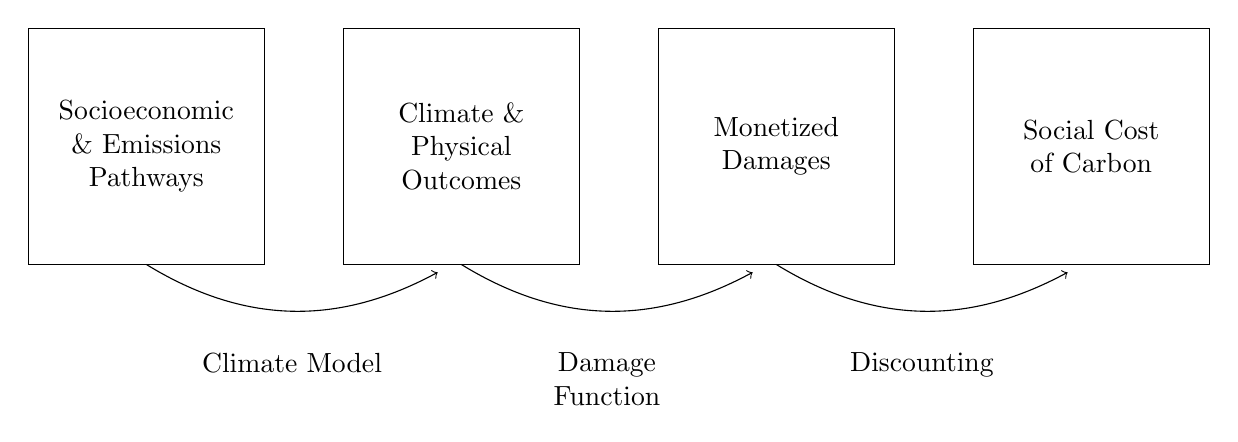
\begin{tikzpicture}
		\draw (0,0) rectangle (3,3) node[pos=0.5, text width=2.5cm, align=center]{Socioeconomic \& Emissions Pathways};
		\draw (4,0) rectangle (7,3) node[pos=0.5, text width=2.5cm, align=center]{Climate \& Physical Outcomes};
		\draw (8,0) rectangle (11,3) node[pos=0.5, text width=2.5cm, align=center]{Monetized Damages};
		\draw (12,0) rectangle (15,3) node[pos=0.5, text width=2.5cm, align=center]{Social Cost of Carbon};
		\draw[->] (1.5,0) to [bend right] (5.2,-0.1);
		\draw[->] (5.5,0) to [bend right] (9.2,-0.1);
		\draw[->] (9.5,0) to [bend right] (13.2,-0.1);
		\node[text width =2.5cm, align=center, below] at (3.35, -1) {Climate Model};
		\node[text width =2.5cm, align=center, below] at (7.35, -1) {Damage Function};
		\node[text width =2.5cm, align=center, below] at (11.35, -1) {Discounting};
	\end{tikzpicture}
	\vspace{1em}
	\fignote[1]{
		Figure adapted from the decriptions in \cite{scc_explainer}, \cite{rennert2022comprehensive}, and \cite{carleton2022guide}. The boxes in the figures display model inputs and outputs, including intermediate inputs and outputs. The arrows, as well as the first box, form what are commonly known to be the four ``modules'' of an IAM.
	}
\end{figure}

In the language of economists, the social cost of carbon looks at the impact of an additional metric ton of carbon dioxide emissions \emph{all else equal}. The first step in the modeling process then is to establish what ``all else" is equal to. Starting from the left side in Figure \ref{scc_visual}, researchers input projections of greenhouse gas emissions and key socioeconomic factors. For instance, the GIVE IAM takes probabilistic projections of emissions for the three major greenhouse gases (carbon dioxide, methane, and nitrous oxide), global population, and per capita economic growth \citep{rennert2022comprehensive}. Researchers take care developing these scenarios in a way that ensures they are internally consistent.\footnote{The creation of these scenarios is often left to a separate class of IAM known as a process-based IAM. The chapters that follow will assume an understanding of the SCC, so this discussion focuses on aggregative IAMs that allow the estimation of the SCC rather than the process-based IAMs used to construct the socioeconomic and greenhouse gas concentration pathways.} The IPCC has standardized a collection of these projections of emissions and socioeconomic variables called the Shared Socioeconomic Pathways (SSPs).\footnote{These SSPs are numbered and often appear in figures that display responses to climate change. For example, consider ``SSP5-8.5.'' The first number, `5' in this case, indicates the SSP scenario.There are five SSP scenarios, each corresponding to a different narrative framing of the response to climate change. In this case, SSP5 is the ``Fossil-fueled Development" pathway, representing a scenario where governments ignore climate damages and attempt to use fossil fuels as a way to develop fast enough to fully adapt to a changing climate \citep{hausfather2018explainer}. The second number is the expected radiative forcing by 2100. In this case, the expected radiative forcing by 2100 is 8.5 W/m$^2$ by 2100. SSP5-8.5 is commonly used as the ``do nothing'' scenario. This notation is similar for Representative Concentration Pathways (RCPs).} With the socioeconomic-emissions pathway set, IAMs simulate two alternative universes: one with an extra emissions pulse in a specified year and one without that emissions pulse. The comparison of damages between these two universes is describes the additional cost of the emissions pulse. In practice, IAMs never just consider a single socioeconomic-emissions pathway, but explore a wide distribution of these pathways.

Next, IAMs map these socioeconomic-emissions pathways to physical impacts. The limitations of the modeling environment mean that IAMs cannot consider all the physical and climatic outcomes that might change as a result of an incremental emissions pulse. Still, IAMs can consider some of the most significant changes in physical outcomes including changes in greenhouse gas concentrations (rather than emissions), temperatures, sea levels, and ocean acidity \citep{sccdatatool}. As Figure \ref{scc_visual} illustrates, IAMs rely on climate models to map an emissions pulse given a socioeconomic-emissions pathway to predict the climate and physical outcomes. Climate scientists would usually predict resulting changes in these variables using a set of models known as General Circulation Models (GCMs). The advantage of GCMs is that they structurally model the mechanisms behind changes in the key physical outcomes. The disadvantage of GCMs is that they are computationally intensive, making them impractical when researchers need to consider a wide distribution of inputs. In practice, researchers use reduced-form versions of GCMs which can capture much of the accuracy of GCMs without all the thermodynamics.

Estimating the changes in the physical environment attributable to an emissions pulse is valuable, but this alone cannot produce a single aggregated impact measure. To produce this measurement, researchers next need to place a dollar value on these physical changes. Economists map physical changes in the climate to dollar values using damage functions, as shown in figure \ref{scc_visual}. The earliest IAM, DICE, utilizes a simple quadratic damage function, calibrated on sums of damage estimates from the IPCC. More contemporary IAMs (e.g., GIVE, FUND, PAGE) contain more sophisticated damage functions that focus on specific damage sectors and calibrate structural economic models to predict sectoral damages given socioeconomic and physical outcomes \citep{national2017valuing}. 

\cite{auffhammer2018quantifying} notes that perhaps the greatest difficulty in using damage functions to map climatic scenarios into physical impacts is accounting for adaptation. To illustrate this, consider Auffhammer's example of air conditioning. Suppose researchers want a damage function to measure the impact of climate change on electricity use. In general, they can expect that consumers will rely more on air conditioners in a warming climate. The response on the intensive margin is measurable. Using data on daily air conditioner use and daily temperatures for instance, researchers could estimate how warming temperatures affect air conditioner use \emph{for those who already have an air conditioner}. Unfortunately, predicting the response in air conditioner adoption and use for those who do not already have a air conditioner---the extensive margin---is much more difficult. This requires data on air conditioner adoption prior to and during anthropogenic climate change, as wells as a strong empirical strategy.\footnote{A promising but limited approach to studying climate change adaptation is by estimating how people have adapted to climate changes in the past. For instance, \cite{druckenmiller2023air} are using historical aerial photographs of Western Africa to study land use and migration changes that occurred as a result of drought during the mid-twentieth century.} Although \cite{auffhammer2018quantifying} provides some guidance, it is clear that accounting for adaptation in damage functions is still an issue. 

\cite{auffhammer2022more} notes that a major focus of future IAMs will be calibrating and incorporating a more comprehensive set of sectoral damage functions. For instance, GIVE currently includes just four sectors in its damage function: agriculture, energy, mortality, and sea level rise. This research need presents a new opportunity for environmental economists to blend their traditional goals of pricing environmental goods with the contemporary tools of applied econometrics. For instance, \cite{druckenmiller2020tree} uses an instrumental variables approach that leverages the sensitivity of bark beetles to temperature shocks to place a value on changes in tree mortality rates. Similar research approaches will be important as economists attempt to incorporate more comprehensive damage functions into IAMs. 

With a monetized pathway of damages, the final task of an IAM is to relate all these future damages back into present terms through a process called discounting. By converting the stream of future damages into present terms, economists can directly compare the current costs of climate action against the future costs of climate inaction. The key parameter in this conversion is called the \emph{discount rate}, $r$. The equation below specifies how the discount rate $r > 0$ relates damages that occur $n$ years in the future back into present terms:
\begin{equation*}
	\text{Present Value of Future Damages} = \left(\frac{1}{1 + r}\right)^n \times \text{Future Damages}.
\end{equation*}
All else equal, the present value of future damages is low when the discount rate is high, and the present value of future damages is high when the discount rate is low.

Discounting is among the most controversial aspects of the cost-benefit approach at the core of IAMs and the SCC, raising serious ethical questions related to intergenerational equity. This is especially contentious when coupled with techniques to assess the value of mortality changes. For instance, if changes in the mortality rate were the only effect of climate change and changes in income over time were ignored, a discount rate of 5\% would imply that 1 life today is equivalent to 100 lives 95 years in the future. This extreme example illustrates why discounting proves to be a controversial yet standard component of the cost-benefit framework behind the SCC. The choice of a discount rate is difficult not only because of the apparent ethical issues with devaluing future generations relative to the current generation, but because the final SCC is highly sensitive to the discount rate. This follows from the long-lived effects of greenhouse gases in the atmosphere.

\cite{carleton2022guide} describe the two primary justifications for a non-zero discount rate. First, a dollar of damages today will be relatively less expensive than a dollar of damages in the future, even when adjusting for inflation. This is because by just about any serious projection, the income per person will be higher in the future. The declining marginal value of consumption means that current costs will be less painful in the future when there is more income to cover them. The second justification for a non-zero discount rate relies on what economists call the \emph{pure rate of time preference}. This says that even with fixed incomes over time, people still value current consumption more than future consumption. In the context of climate damages, this is often quite contentious. At a minimum, assigning a parameter value such that a human life in the future is not worth as mush as a human life today inherently feels wrong. Carleton and Greenstone offer that even in the case of human life, a pure rate of time preference might be justified considering the non-zero probability of apocalyptic events like an asteroid strike or nuclear war. With this interpretation, it is not that we value human life in the future less than today necessarily, but that we never know if there will be a future. 

Even if researchers rule out a discount rate of zero, the choice of discount rate is still highly ambiguous. There are two primary approaches to identifying the ``correct'' discount rate. The first sets the discount rate equal to the rate of return for capital assets. The motivation for choosing the discount rate to match the rate of return for capital assets follows neatly from Robert Solow's definition of sustainability: ``[sustainability is] an obligation to conduct ourselves so that we leave to the future the option or the capacity to be as well off as we are'' \citep{solow1991sustainability}. Setting the discount rate equal to the rate of return for capital assets presumably ensures that future generations will be indifferent between current investments to reduce future climate damages and any other current investment that would compensate for these damages (a no arbitrage condition). Typically, economists consider the US Treasury Bonds to be the appropriate benchmark capital asset. Recent analysis finds that the Treasury Inflation-Indexed Security had average annual returns of just 1.01\% from 2003 (when data are first available) through 2021. Of course, this approach lends itself to criticism surrounding uncertainty in future US Treasury yields. 

A second approach to the discount rate comes through \cite{ramsey1928mathematical}. This paper lays the foundation for what is now known as the Ramsey equation:
\begin{equation*}
	r = \delta + \eta g
\end{equation*}
where $r$ is the discount rate, $\delta$ is the pure rate of time preference, $\eta$ represents the elasticity of the marginal utility of consumption, and $g$ is the real growth rate of consumption. The Ramsey equation is useful in IAMs in that it treats the discount rate as endogenous to the socioeconomic pathway given, providing an additional level of internal consistency. However, uncertainties around the growth rate of consumption present difficulties for Ramsey-style discounting \citep{national2017valuing, newell2022discounting}. Additionally, estimating the key parameter values often rely more on expert elicitation rather than clear derivations from market data, which is not always appealing.

In its authors' preferred specification, GIVE uses a discount rate of 2\%. This is consistent with \cite{carleton2022guide}, who recommend a discount rate of at most 2\%. Increasingly, a discount rate centered around 2\% appears to be the norm in SCC estimation. 

The reality of policy design in the US requires cost-benefit analysis for environment and climate policy. Regardless of whether or not this is the ideal framework to use when crafting climate policy, IAMs and their ability to connect current economic activity directly to future climate damages will remain an important tool in developing climate policy. There is still considerable room for economists to advance our understanding of the implications of climate change going forward. What we do know is that today, our best estimates indicate that the impacts of climate change are troubling. 

% In general, placing a dollar value on climate damages is understandably controversial, particularly when the damages involve changes in mortality rates.\footnote{See \cite{colmer2020meaning} for a recent and careful review of this issue outside of climate policy.}

% While these process-based models create the backbone of impact estimates, economists often opt to use simpler method for mapping climatic outcomes to quantitative impacts called damage functions. Damage functions are reduced-form estimations of the relationship between climate variables (e.g. average surface temperatures) and impact variables of interest (e.g. mortality rates). That is, damage functions do not attempt to explain the complex systems that give rise to these damages and focus instead on just explaining aggregate impacts. For instance, [CITATION] create straightforward damage functions for the US by using process-based impact models to generate estimates of climate change impacts (in monetary terms) under a variety of climate scenarios. Then they use OLS to estimate the relationship between surface temperature measurements and the monetary value of climate change impacts. The estimated model is a damage function, mapping changes in surface temparatures to impacts. Damage functions like this and many others provide useful tool in a variety of applications, especially in calculating the social cost of carbon. 

% Admittedly, there is a considerable amount we still do not know about the impacts of climate change. Truthfully, we are not exactly sure how the estimated 3.3 to 3.6 \emph{billion} people who are highly vulnerable to climate change will adapt [CITATION]. Will hundreds of millions of people living in some of the most impoverished corners of the planet seamlessly migrate en masse to places with more hospitable climates over the course of just a few decades? 

% intramarginal vs. extramarginal

% While many systems---both natural and social---face steep challenges from climate change, some of these face complete ruin. Many of the most vulerable systems are endemic. Endemism refers to species, cultures, and resources that are restricted to specific geographic areas. [CITATION] In a changing climate, systems that are tied to specific regions and climates risk extinction if they cannot plausibly adapt. This includes the extinction of species whose habitats are destroyed by climate change, 
% the death of indigenous cultures that are highly dependent on the climate, and the destruction of historical artifacts and landmarks. Unfornately in each of these cases, the affected system cannot is unique and we could not replace it for the remainder of human existence. These kind of consequences do not fit well into standard economic understanding of sustainability. \footnote{*Talk about an economic definition of sustainability from Romer, and why it might not be able to capture some of the threats of climate change well.*}


%%%%%%%%%%%%%%%%%%%%%%%%%%%%%%%%%%%%%%%%%%%%%%%%%%%%%%%%%%%%%%%%%%%%
%\subsection{The Impact of Climate Change}
%
%At this point we have covered why we know climate change exists, why we know humans are responsible for climate change, and what the composition of greenhouse gas emissions look like. We have to to justify why anyone should care about climate change though. Here, we take a brief and high-level examination of the impacts of climate change. If I had to summarize the magnitude of climate impact estimates by even just the end of the century, I would probably say that they lie somewhere in between pretty bad to borderline apocalyptic. 
%
%Admittedly, the impacts of climate change on natural ecosystems and society are not understood quite as well as the causes of climate change. This gap in knowledge is closing as we collect new data on the impact of the climate change we have already seen. The IPCC summarizes these impacts in its Fifth Assessment Report in five ``reasons for concern." These reasons for concern relate to:
%\begin{enumerate}
%	\item Unique and threatened systems
%	\item Extreme weather events
%	\item Distribution of impacts
%	\item Global aggregate impacts
%	\item Large-scale singular events
%\end{enumerate}
%
%There are certain physical elements of the natural and built environment that are unique and irreplaceable. Losing these due to climate change poses a significant cost for all future generations. For instance, warming waters threatens coral reefs. With sustained and substantial warming, the world's coral reefs could be permanently destroyed. Many important historical sites are located in low-lying coastal areas threatened by rising sea levels from climate change. Climate change has the power to permanently destroy many of the ecosystems we cherish and other culturally significant creations.
%
%Extreme weather events pose the greatest This includes a greater frequency of severe but short-lived weather events, like tornadoes or monsoons. More concerning is are sustained heat-stress events. As Freddy's mom from iCarly once said, ``when temperatures get too high, the elderly will start to die" (a rather creepy but fitting rhyme). Elevated temperatures can induce cardiovascular events, particularly in vulnerable populations like the poor, elderly, and those who work outside. Sustained events like this can trigger droughts and resulting in famine. Higher humidity can bolster mosquito populations and allow blood-borne infectious disease to spread easier. Extreme and sustained events like these pose serious challenges to public health.
%
%Related to this, impacts tend to fall most severely on populations who are already at the greatest disadvantage. Some of this is simply due to geography. Climate predictions for the African continent are sickening. Much of this is due to adaptation costs. When it is 110$^\circ$F outside, the well off do not just sweat---they run their air conditioners on full blast. This is not true of the global poor, who cannot afford to pay to adapt to rising temperatures, and instead suffer the heat and risk death. 
%
%Global impacts on natural life and the economy are not well understood, but what we know is not reassuring. The economic impacts of climate change will become much more apparent as concentrations of greenhouse gases increases. That is, the economic damages from climate change are increasing at an increasing rate with the concentration of greenhouse gases. There is some additional concern about low-probability, highly dangerous climate change-induced events. 
%
%\begin{figure}
%	\caption{Climate Change Damages by Income \& Climate \citep{carleton2020valuing} \label{cil1}}
%	\centering
%	\includegraphics[width = \textwidth]{figures/chapter1_figures/cil_dist.png}
%\end{figure}
%
%\begin{figure}
%	\caption{The Climate Change Mortality Rate \citep{carleton2020valuing} \label{cil2}}
%	\centering
%	\includegraphics[width = 0.8\textwidth]{figures/chapter1_figures/cil_mortal.png}
%\end{figure}
%
%Figures \ref{cil1} and \ref{cil2} depict estimates of moralities by end of the century from climate change induced events. These summarize many of the most important takeaways from the impacts of climate change. Those who live in poor and warm areas will suffer the most from climate change. The mortality rate from climate change is comparable to the mortality rate of other leading causes of death. Overall, the situation climate change poses by just the end of the century is extremely grim and warrants sweeping action.